\chapter{Memory Model-Awared Program Analysis}
\label{ch:wmm}

In general, analysis of concurrent programs with respect to axiomatic memory models require firstly to capture the control-flow of a concurrent program, after which the set of all possible data-flows (called \textit{candidate executions}) is computed as the set of possible communications between threads of the program. After that, the \textit{weak memory model} specification constraints this set of candidate executions and decides which execution is valid~\cite{alglave2014herding}.
More specifically, we use the event-based program representation (see Section~\ref{ch:wmm:model:events}) as a natural way to capture the semantics of a concurrent program. Therefore, a candidate execution is defined as a choice of events to be executed. The constraints over events imposed by both program and memory model are called \textit{relations} (see Section~\ref{ch:wmm:model:relations})

%More presice description of x86-TSO memory model is given in Chapter~\ref{ch:wmm:x86}.

\section{The event-based program representation}
\label{ch:wmm:event}

%"The semantics of a program is a set of executions" https://johnwickerson.github.io/papers/memalloy.pdf

The classical approach to model concurrent programs is to use the \textit{global time}, a single order of interleavings of all actions happened in different threads. However these models are easy to understand, it may be hard to consider \textit{all} possible states, number of which is exponentially large. Another way to do this is to to use non-deterministic computation-centric models defined in~\cite{fri97}, one of which represents the program as the graph of \textit{memory events}. The idea in this class of models is based on the fact that the behaviour of a concurrent system is defined only by the interleavings of shared-memory operations, while being independent from the order of local computation events.
%These models may be further restricted by constraints of a weak memory model, adding \textit{relations} to the memory events.
%Perhaps, the most convenient way to model the non-deterministic properties of concurrent programs is to use the program representation based on \textit{memory events}.
%In order to model the non-deterministic properties of concurrent programs 

The event-based program model represents the directed graph (the \textit{event-flow graph}), where vertices represent \textit{events} (simple low-level instructions), and edges represent \textit{relations} over the events.
Below we describe some basic types of events and relations.

\subsection{Events}
\label{ch:wmm:model:events}

A \textit{memory event} $e_m \in \mathbb{E}$ represents the fact of access to the memory. Since memory is the crucial low-level resource shared by multiple processes, most relations are defined over memory events. 
The processes can access a shared memory location (denoted by~$l_i$, for \textit{location}), or a local one (denoted by~$r_i$, for \textit{register}). A memory event can access at most one shared memory location, high-level instructions that address more than one shared variable must be transformed into a sequence of events. A memory event is specified by its direction with respect to the shared variable, its location~$\mathtt{loc}(e_m)$, its processor label~$\mathtt{proc}(e_m)$, and a unique event label~$\mathtt{id}(e_m)$~\cite{alglave2010shared}. 
%\texttt{load} for read the value of a shared-memory location, or \texttt{store} for write, or neither of them if both locations are local
The set of memory events $\mathbb{M}$ is devided into write events $\mathbb{W}$ (that write values to shared-memory locations) and read events $\mathbb{R}$ (that read values stored in shared-memory locations).
We add a restriction that each memory event uses at most one shared location, so that the write event $e_m = write(l_1, l_2)$ that writes value from shared location $l_2$ to the shared location $l_1$ is represented as two consequent events $e_m'~=~\mathtt{load}(r_1 \leftarrow l_2); \ e_m''~=~\mathtt{store}(l_1 \leftarrow r_1)$.

A \textit{computation event} $e_c \in \mathbb{C} \subseteq \mathbb{E}$, represents a low-level assembly computation operation performed solely on local-memory arguments. An example of computation event may be the event $e_c = r_1 \leftarrow add(r_2, 1)$ that writes the sum of values stored in register $r_2$ and constant $1$ (emulated as a register as well) to the register $r_1$. For modelling branching statements, we distinguish the set $\mathbb{C_{p}} \subseteq \mathbb{C}$ of \textit{predicative} computation events, that are evaluated as a boolean value.%TODO: TAUTOLOGY HERE.

The third class of events is \textit{barrier events}, events caused by the synchronisation instructions (called \textit{fences}). Barrier events do not perform any computation or memory value transfer, instead, they add new relations to the program model that restrict the set of allowed behaviours. Technically, a fence may be represented either as a synchronisation barrier, or a flush local memory caches, etc.


\subsection{Relations}
\label{ch:wmm:model:relations}

In this section, we describe basic derived relations used in memory model-awared program analysis.

%The \textit{control-flow} instructions (conditional and unconditional jumps) are encoded into the model directly, without additional events, as the $po$-relation (for \textit{program order}; see Chapter~\ref{ch:wmm:model:relations} for detailed definition of relations).
The \textit{control-flow} of a program is defined by \texttt{po}-relation $\subset~\mathbb{E}~\times~\mathbb{E}$ (\textit{program-order}), which represents the total order of events \textit{from same process}, which never relates events from different processes.
Thus, if a program specifies the memory instruction $i_2$ to follow immideately the memory instruction $i_2$, then there exist an edge $e_1 \xrightarrow{\mathtt{po}} e_2$ in the event-flow graph where event $e_1$ is caused by the instruction $i_1$ and $e_2$ is caused by the instruction $i_2$. This relation encodes the control-flow of the program into the event-flow graph.
%Some new relations may be acquired : dp, po-loc

The \textit{data-flow} of a program is defined by \textit{communication relations}: the \rf-relation $\subset~\mathbb{W}~\times~\mathbb{R}$ (\textit{read-from} relation) that maps a write event to the read event that reads its value, the \co-relation $\subset~\mathbb{W}~\times~\mathbb{W}$ (\textit{coherence order}, sometimes called \texttt{ws}-relation for \textit{write serialisation}) defines the total order on writes to the same location across all processes, and the \fr-relation $\subset~\mathbb{R}~\times~\mathbb{W}$ (\textit{from-read order}) that maps a read to possible writes preceding the current write event (this relation is the inversion of the \rf-relation: $\mathtt{rf} = \mathtt{fr}^{-1}$).
%TODO: perephrase last sentence! alglave thesis, p. 36

\subsection{Executions}
\label{ch:wmm:model:executions}

The semantics of a concurrent program is represented by the set of allowed executions.
A \textit{candidate execution} (trace, run) of a program is an ordered set of events defined by \po and \rf relations and set of final writes to a given memory location~\cite{alglave2014herding}.
%The order of events in particular execution is denoted as `$\rightarrow$', an empty execution is denoted as $\emptyset$.

%associated with the instructions of the program
%the path in the event-flow graph. 
An execution is considered to be \textit{valid} if the memory events follow a single global timeline, textit.e., can be embedded in a single partial order allowed by the memory model restrictions~\cite{alglave2010shared}. 
An execution to be checked on validity is called the \textit{candidate execution}.
An execution is uniquely defined by the set $\mathbb{X}$ of events have been executed in each thread (the \textit{control-flow} of a program), and the relations $\mathtt{rf}$ and $\mathtt{co}$~\cite{alglave2010shared}.
As it was shown in~\cite{wickerson2017automatically}, it is enough for memory models to constrain the executions independently instead of constraining the program as a whole.
Figure~\ref{simple_wmm_x86_pic} illustrates four possible candidate executions for the litmus-test Example~\ref{simple_wmm_x86} (the pictures are generated by the \texttt{herd7} tool, version 7.47). Since there are no conditional jumps, the \po-relation is defined and we do not need to guess it. Since each thread performs single write followed by a single read, the \co-relation is also defined (it relates the initial write event with the write event to the same location). Thus, there are only four possible executions defined by the choice of \rf-relation. The candidate executions pictured in Figures~\ref{simple_wmm_x86_pic:sub1}--\ref{simple_wmm_x86_pic:sub3} are consistent both under strong memory model SC and under relaxed memory models x86-TSO, Power, ARM, and others. However, the execution shown in Figure~\ref{simple_wmm_x86_pic:sub3} is still consistent under relaxed-memory architectures, but it becomes inconsistent under SC architecture as it forbids cycles over \fr$\cup$\po.
%The event $b$:\texttt{(Ry=0)} reads value \texttt{0} at the shared location \texttt{y} from the initial write event $e$\texttt{(Wy=0)} (the red edge of \texttt{rf}-relation), consequently, 
%the event $d$:\texttt{(Rx=0)} reads value \texttt{0} at the shared location \texttt{x} from the initial write event $f$\texttt{(Wx=0)} (the red edge of \texttt{rf}-relation). 
%However, the Power memory model allows such cycles, therefore %TODO: include load buffering example, see presentation pdf

%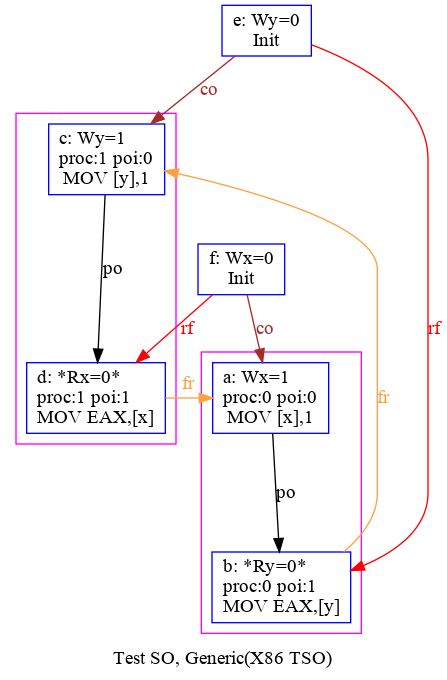
\includegraphics[width=0.4\textwidth]{img/my/simple_wmm_x86.png}
\begin{figure}
\centering
\begin{subfigure}[t]{.28\textwidth}
  \centering
  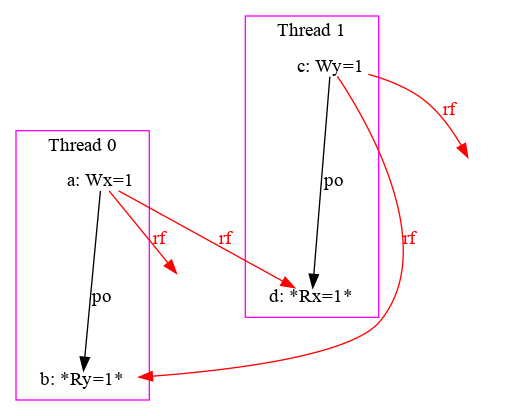
\includegraphics[width=1.2\linewidth]{img/my/sb-example/SB-dot.png}
  \caption{Final state: \texttt{(0:EAX=1~/\textbackslash~1:EAX=1)}}
  \label{simple_wmm_x86_pic:sub1}
\end{subfigure}
\hfill
\begin{subfigure}[t]{.23\textwidth}
  \centering
  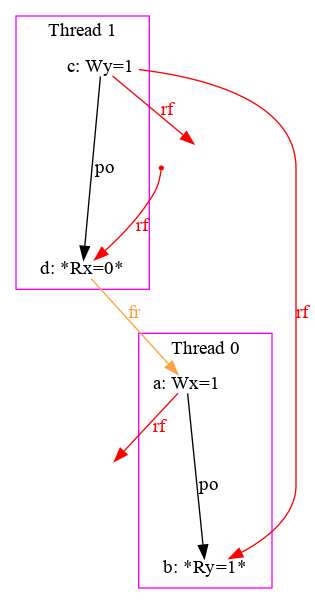
\includegraphics[width=.9\linewidth]{img/my/sb-example/SB-dot-2.png}
  \caption{Final state: \texttt{(0:EAX=1~/\textbackslash~1:EAX=0)}}
  \label{simple_wmm_x86_pic:sub2}
\end{subfigure}
\hfill
\begin{subfigure}[t]{.23\textwidth}
  \centering
  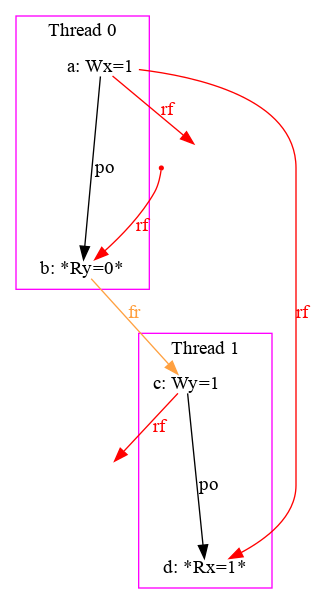
\includegraphics[width=.9\linewidth]{img/my/sb-example/SB-dot-3.png}
  \caption{Final state: \texttt{(0:EAX=1~/\textbackslash~1:EAX=1)}}
  \label{simple_wmm_x86_pic:sub3}
\end{subfigure}
\hfill
\begin{subfigure}[t]{.23\textwidth}
  \centering
  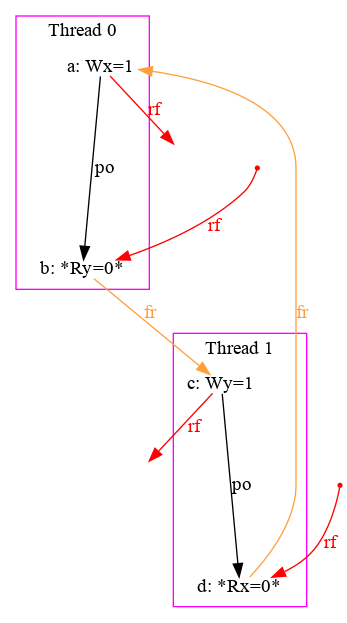
\includegraphics[width=.9\linewidth]{img/my/sb-example/SB-dot-4.png}
  \caption{Final state: \texttt{(0:EAX=0~/\textbackslash~1:EAX=0)}}
  \label{simple_wmm_x86_pic:sub4}
\end{subfigure}
\hfill
\caption{Candidate executions for the litmus test Example~\ref{simple_wmm_x86}}
\label{simple_wmm_x86_pic}
\end{figure}



\section{The CAT language}

One common way to define a weak memory model in a systematic way in to formalise it in \textit{the CAT language} proposed in~\cite{alglave2016syntax}. The CAT language allows to axiomatically define new relations, new fences and restrictions over relations.


%// exmaple with reordering
%// ex. with 
%// Rev-29 Example 7-6. Stores Are Transitively Visible. %see http://www.cl.cam.ac.uk/~pes20/weakmemory/x86tso-paper.pdf

%There is a barrier instruction \texttt{mfence} that may be used for flushing the buffers into the main memory.

briefly some hw memory models: X86-TSO, Alpha, POWER, ;

language memory models: Java, C++;

library-level kernel memory model, ref to github with tests

%Relationship between different models \url{http://wiki.expertiza.ncsu.edu/index.php/CSC/ECE_506_Spring_2013/10c_ks}


\section{Some examples of WMM}

//axioms of TSO wmm

// example of sets: rf, co, ... for the code snipped used before

